%https://tex.stackexchange.com/q/737612/86
\documentclass[tikz,border=5pt]{standalone}
\usetikzlibrary{intersections,spath3}
\begin{document}
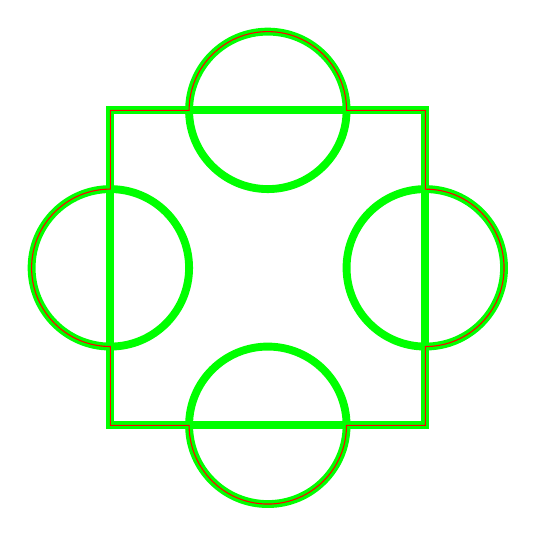
\begin{tikzpicture}
\path[draw,green,line width=1mm,spath/save=S] (-2,-2) rectangle (2,2);
\path[draw,green,line width=1mm,spath/save=A] (0,2) circle[radius=1];
\path[draw,green,line width=1mm,spath/save=B] (2,0) circle[radius=1];
\path[draw,green,line width=1mm,spath/save=C] (0,-2) circle[radius=1];
\path[draw,green,line width=1mm,spath/save=D] (-2,0) circle[radius=1];
        
\tikzset
{%定义交点与路径分段
  spath/split at intersections={S}{A},
  spath/split at intersections={S}{B},
  spath/split at intersections={S}{C},
  spath/split at intersections={S}{D},
  spath/get components of={A}{\Acpts},
  spath/get components of={B}{\Bcpts},
  spath/get components of={C}{\Ccpts},
  spath/get components of={D}{\Dcpts},
  spath/get components of={S}{\Scpts},
}

\path[spath/save=Union,
  spath/use={\getComponentOf\Acpts{2},reverse},
  spath/use={\getComponentOf\Scpts{3},weld},
  spath/use={\getComponentOf\Bcpts{3},reverse,weld},
  spath/use={\getComponentOf\Scpts{5},weld},
  spath/use={\getComponentOf\Ccpts{3},reverse,weld},
  spath/use={\getComponentOf\Scpts{7},weld},
  spath/use={\getComponentOf\Dcpts{2},reverse,weld},
  spath/use={\getComponentOf\Scpts{9},weld},
  spath/adjust and close=current
];

\draw[red,spath/use=Union];
\end{tikzpicture}

\begin{tikzpicture}
\path[spath/save=P] 
    (-2,2) -- (-1,2) arc(180:0:1cm) 
    -- 
    (2,2) -- (2,1) arc(90:-90:1cm) 
    -- 
    (2,-2) -- (1,-2) arc(360:180:1cm) 
    -- 
    (-2,-2) -- (-2,-1) arc(270:90:1cm) 
    -- cycle;
\draw[spath/use=P];
\end{tikzpicture}

\end{document}